\begin{frame}{\insertsection}
\begin{columns}
\column{.45\textwidth}
	\begin{itemize}
	\item blind detection is used
	\item estimation of $\mu_i$ and $\sigma_i$ from watermarked image:
	\end{itemize}
	\begin{align*}
	\hat{\mu}_i &= \frac{1}{N_B} \sum_{y \in B}y\\
	\hat{\sigma}_i^2 &= \frac{1}{N_B - 1} \sum_{y\in B}(y-\hat{\mu}_i)^2
	\end{align*}
where $y$ is the corresponding DWT coefficient of the watermarked image
\column{.45\textwidth}
	\begin{figure}
	\centering
	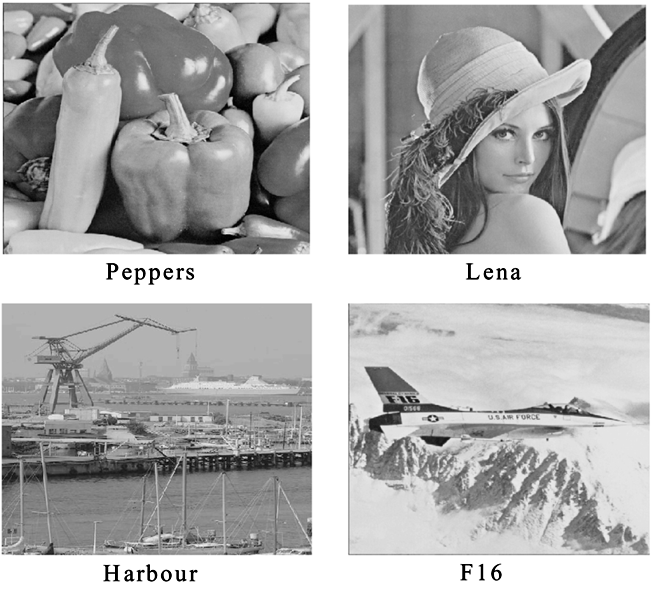
\includegraphics[width=\textwidth]{Bilder/ResultsBilder} 
	\end{figure}
	\end{columns}
\end{frame}

\begin{frame}{\insertsection}

	Three tested image processing operations:
	\vspace{2mm}
	\begin{enumerate}
	\item JPEG compression with $50\%$ quality factor
	\item blurred, using $4 \times 4$ spatial filter
	\item corrupted by Gaussian noise with $\mu = 0$ and $\sigma^2 = 0.5$ 
	\end{enumerate}
	\vspace{5mm}
	\textcolor{TUDblue}{$\Rightarrow$} results are based on 10000 trials \\
	\textcolor{TUDblue}{$\Rightarrow$} in each trial, embedded watermark $\bm w^*$ is chosen from \\ \hspace{3.5mm} a set $W$ of 100 randomly generated watermarks \\
	\textcolor{TUDblue}{$\Rightarrow$} successful detection, if threshold is exceeded for this watermark, \\ \hspace{3.5mm} but not for any other watermark in $W$
	
\end{frame}

\begin{frame}{\insertsection}
\vspace{-6mm}
	\begin{figure}
	\centering
	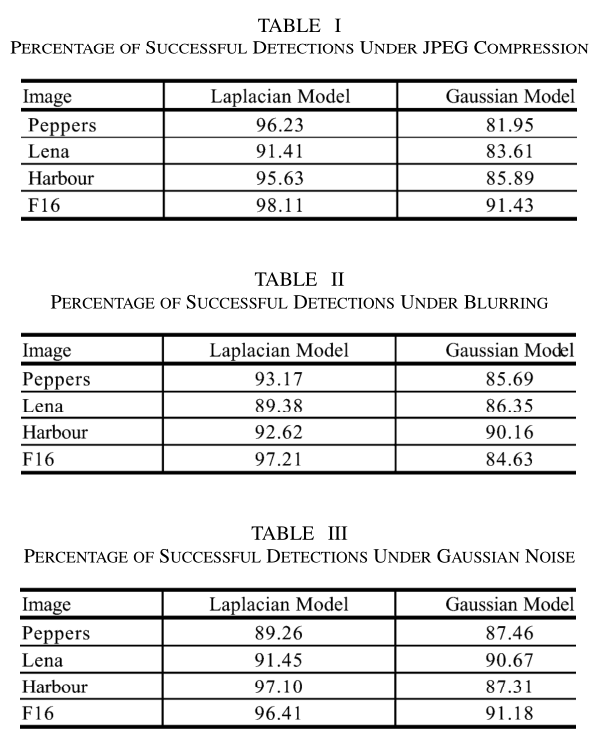
\includegraphics[height=\textheight]{Bilder/tablesall} 
	\end{figure}
\end{frame}